\section{The MorphoPath-Edge Methodology}
\label{sec:methodology}

The architecture of \textbf{MorphoPath-Edge} is illustrated in Fig.~\ref{fig:architecture}. The framework executes across five deterministic, gradient-free stages: (i) dual-stream vision foundation feature extraction; (ii) Tukey ladder-of-powers normalization; (iii) closed-form zero-parameter test-time manifold rectification; (iv) intra-archetype regularized Fisher discriminant analysis coupled with micro-symptom prompt ensembles; and (v) cardinality-equalized Bayesian differential triage.

\subsection{Dual-Stream Feature Extraction and Tukey Normalization}
\label{subsec:dual_stream_tukey}
To decouple macroscopic leaf geometry from microscopic lesion pathology, an input image $x \in \mathcal{X}$ is encoded through two frozen, INT8-quantized vision foundation backbones:
\begin{equation}
    z_{\text{dino}} = f_{\text{dino}}(x) \in \mathbb{R}^{384}, \quad z_{\text{bio}} = f_{\text{bio}}(x) \in \mathbb{R}^{512},
    \label{eq:dual_features}
\end{equation}
where $f_{\text{dino}}$ is DINOv2 ViT-S/14~\cite{oquab2023dinov2}, capturing organ geometry, venation, and leaf margins; while $f_{\text{bio}}$ is BioCLIP ViT-B/16~\cite{stevens2024bioclip}, trained on organismal taxonomies and attuned to necrotic lesions and chlorosis. The representations are concatenated to form an initial joint embedding $z_{\text{joint}} = [z_{\text{bio}}^\top, z_{\text{dino}}^\top]^\top \in \mathbb{R}^{896}$.

To eliminate directional anisotropy and heavy-tailed distribution skew, we apply Tukey's ladder-of-powers transformation~\cite{tukey1977exploratory} ($\beta=0.5$) followed by unit hypersphere projection:
\begin{equation}
    z_{\text{tukey}}^{(d)} = \text{sign}\left(z_{\text{joint}}^{(d)}\right) \cdot \left| z_{\text{joint}}^{(d)} \right|^{0.5}, \quad \hat{z} = \frac{z_{\text{tukey}}}{\| z_{\text{tukey}} \|_2} \in \mathbb{S}^{D-1},
    \label{eq:tukey_transform}
\end{equation}
stabilizing multivariate Gaussianity for subsequent discriminant estimation.

\subsection{Botanical Archetype Routing}
\label{subsec:archetype_routing}
Rather than predicting fragile cultigen species, the query's macroscopic morphology is routed across the four foliar archetypes $\mathcal{A} = \{A_0, A_1, A_2, A_3\}$ using the pathology-invariant representation $z_{\text{dino}}$. For each archetype $A_k$, a normalized centroid $\mu_{A_k}^{\text{dino}} = \text{norm}\left( \frac{1}{|\mathcal{S}_{A_k}|} \sum_{x \in \mathcal{S}_{A_k}} f_{\text{dino}}(x) \right)$ is precomputed. The archetype prior probability is evaluated via temperature-scaled cosine softmax ($T=12$):
\begin{equation}
    P(A_k \mid x) = \frac{\exp\left( T \cdot \cos\left( \text{norm}(z_{\text{dino}}), \mu_{A_k}^{\text{dino}} \right) \right)}{\sum_{j=0}^3 \exp\left( T \cdot \cos\left( \text{norm}(z_{\text{dino}}), \mu_{A_j}^{\text{dino}} \right) \right)},
    \label{eq:archetype_prior}
\end{equation}
achieving 91.39\%--93.25\% accuracy in the wild with 100.00\% Top-2 recall.

\subsection{Closed-Form Zero-Parameter Test-Time Manifold Rectification}
\label{subsec:manifold_rectification}
Under in-the-wild field conditions, illumination and sensor chromaticity induce a systematic translation vector between support and query distributions: $\Delta = \mu_q - \mu_s$, where $\mu_s = \mathbb{E}_{\mathcal{S}}[\hat{z}]$ and $\mu_q = \mathbb{E}_{\mathcal{Q}}[\hat{z}]$, with $\|\Delta\|_2 \in [0.21, 0.30]$ (Fig.~\ref{fig:tsne_rectification}).

\begin{figure}[t]
    \centering
    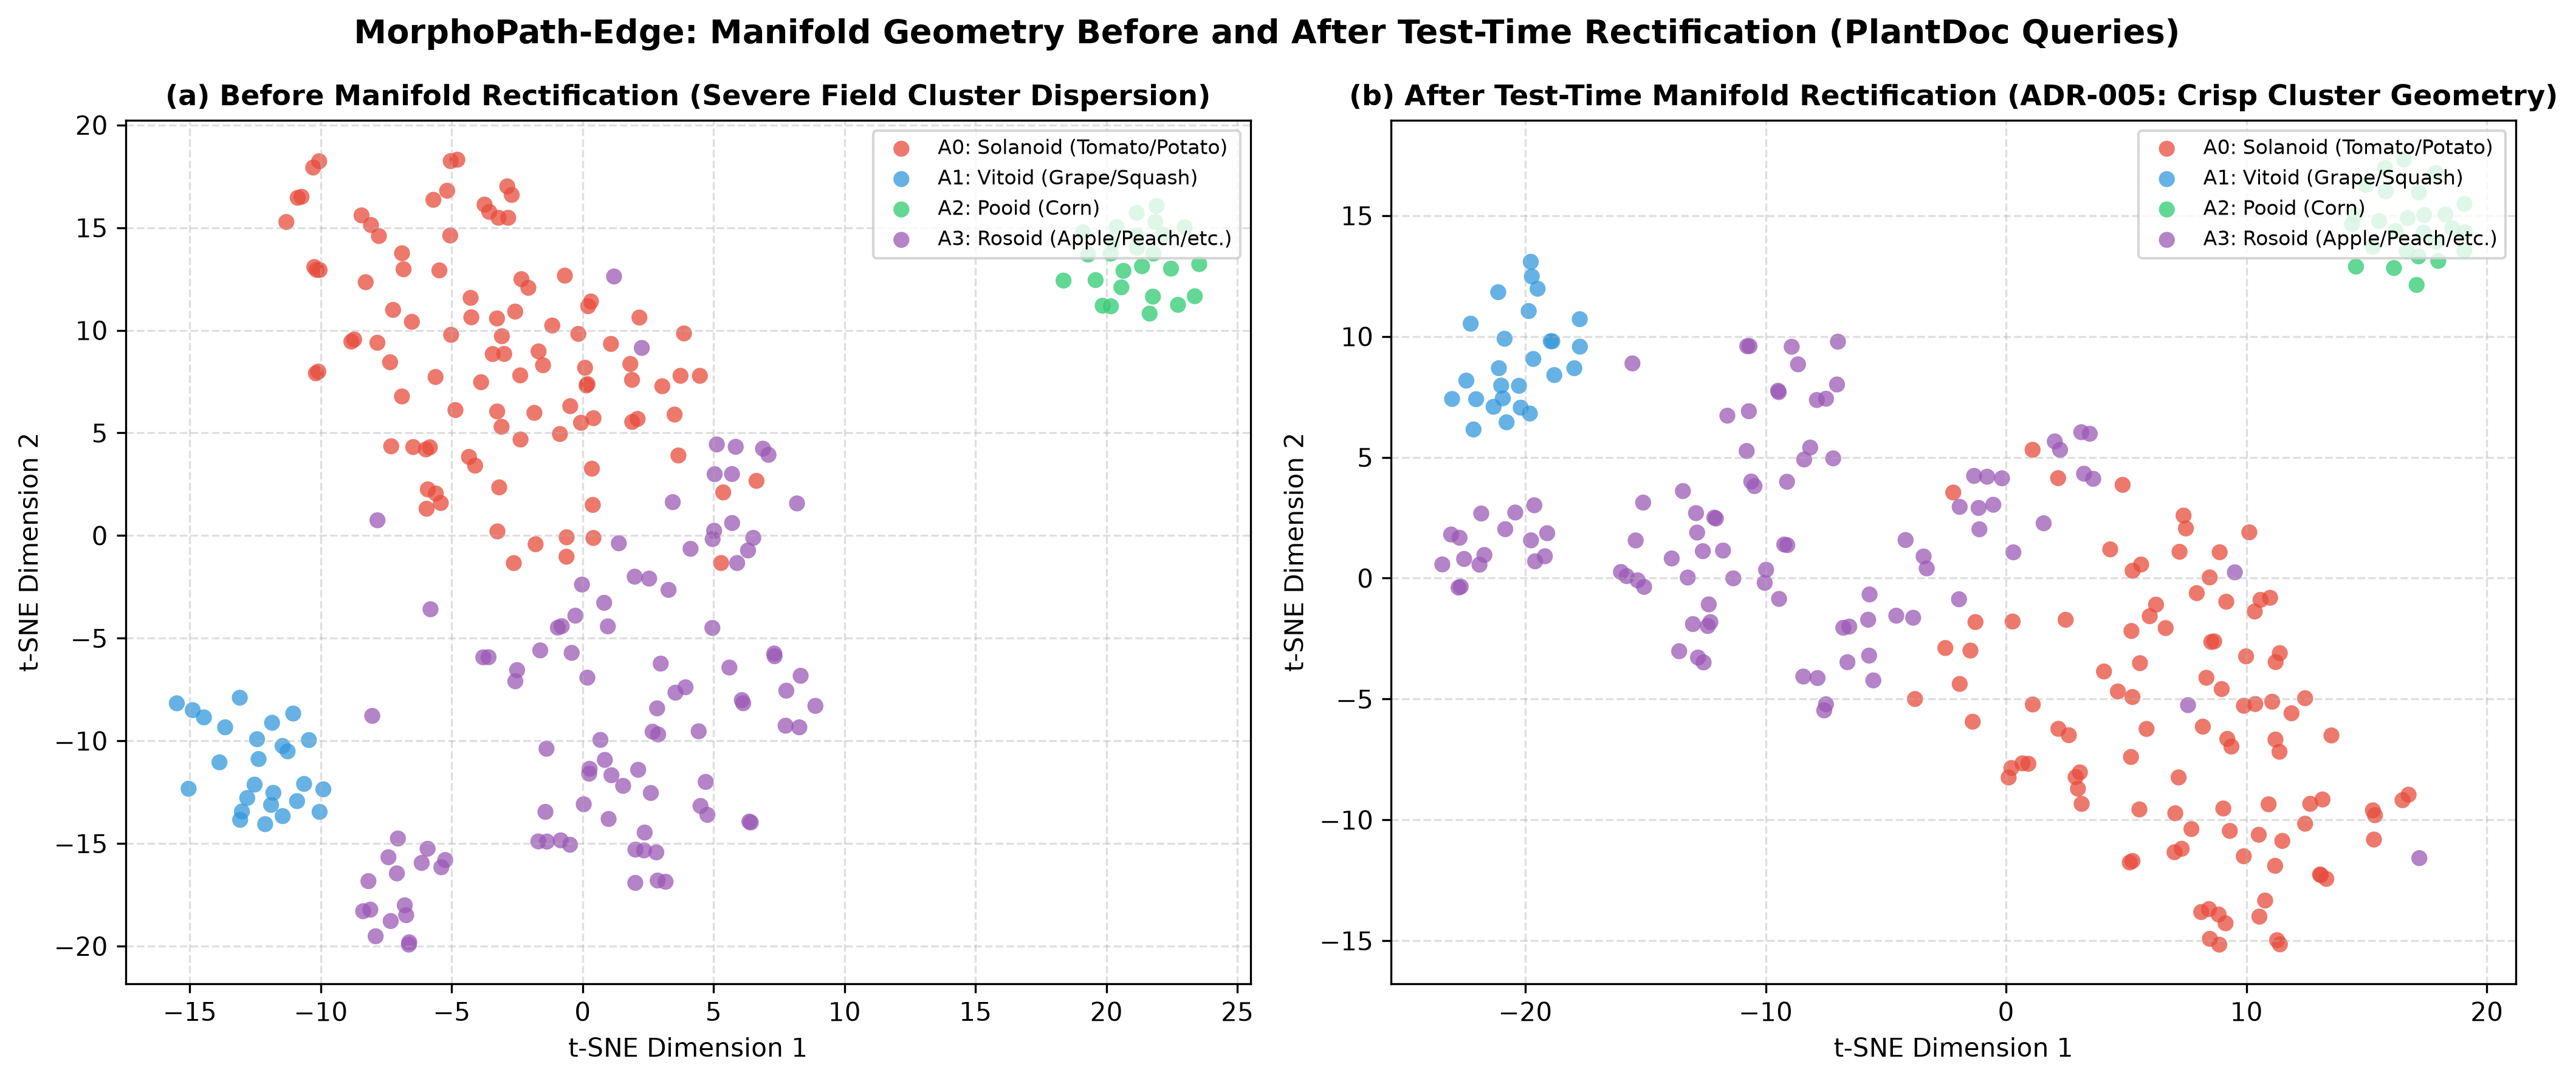
\includegraphics[width=0.82\columnwidth]{figures/tsne_manifold_rectification.png}
    \caption{Visualizing field domain shift and closed-form rectification on PlantDoc. Left: Raw uncalibrated representations exhibit severe systematic centroid drift ($\|\Delta\|_2 \approx 0.30$) between support and query distributions. Right: Our Zero-Parameter Test-Time Manifold Rectification aligns class centroids algebraically without gradient optimization, recovering class separability on resource-constrained edge hardware.}
    \label{fig:tsne_rectification}
\end{figure}

To eliminate $\Delta$ without backpropagation, we formulate \textbf{Zero-Parameter Test-Time Manifold Rectification} (ADR-005):

\noindent\textbf{Proposition 1 (Domain Shift Invariance under Mean Rectification).}
\textit{Let $\hat{z}_s \sim \mathcal{D}_s$ with expectation $\mu_s$, and let field queries experience an additive domain translation $\hat{z}_q \sim \mathcal{D}_q$ with expectation $\mu_q = \mu_s + \Delta$. The centered representations satisfy $\mathbb{E}[\hat{z}_q - \mu_q] - \mathbb{E}[\hat{z}_s - \mu_s] = \mathbf{0}$, algebraically eliminating the first-order translation $\Delta$. Subsequent unit-hypersphere projection:
\begin{equation}
    \tilde{z}_s = \frac{\hat{z}_s - \mu_s}{\| \hat{z}_s - \mu_s \|_2}, \qquad \tilde{z}_q = \frac{\hat{z}_q - \mu_q}{\| \hat{z}_q - \mu_q \|_2},
    \label{eq:centering_transformation}
\end{equation}
aligns the centered support and query distributions onto $\mathbb{S}^{D-1}$ with common origin.}

\textit{Proof.} By linearity of expectation, $\mathbb{E}[\hat{z}_q - \mu_q] = (\mu_s + \Delta) - (\mu_s + \Delta) = \mathbf{0}$ and $\mathbb{E}[\hat{z}_s - \mu_s] = \mathbf{0}$. The common-mode additive shift $\Delta$ is identically canceled prior to angular prototype comparison with zero parameter updates. \hfill $\blacksquare$

Rectified prototypes are then computed as $P_c^{\text{rect}} = \text{norm}\left( \frac{1}{|\mathcal{S}_c|} \sum_{x \in \mathcal{S}_c} \tilde{z}_s(x) \right)$. For continuous streaming, $\mu_q$ is maintained via an online running average: $\mu_q^{(t)} = (1 - \gamma)\mu_q^{(t-1)} + \gamma \hat{z}_q^{(t)}$ with $\gamma = 0.05$.

\subsection{Intra-Archetype Shrunk Fisher LDA and Micro-Symptom Ensembles}
\label{subsec:shrunk_fisher_lda}
Within archetype $A_k$, the support sample count is vastly smaller than the feature dimension ($N_{A_k} K \ll D$, e.g., $50 \ll 896$), rendering the empirical pooled within-class covariance $\Sigma_w^{(k)}$ singular ($\kappa = \infty$). Following Ledoit and Wolf~\cite{ledoit2004well} (ADR-002), we apply analytical covariance shrinkage:
\begin{equation}
    \Sigma_{\text{shrunk}}^{(k)} = (1 - \lambda) \Sigma_w^{(k)} + \lambda \frac{\text{Tr}\left(\Sigma_w^{(k)}\right)}{D} I_D,
    \label{eq:shrunk_cov}
\end{equation}
where $\lambda = 0.60$ reduces the condition number to $\kappa = 1428$. The visual conditional likelihood is evaluated via regularized Mahalanobis distance:
\begin{equation}
    P_{\text{vis}}(c \mid x, A_k) = \frac{\exp\left( -\frac{1}{2} d_{\Sigma}^{(k)}\left(\tilde{z}_q, P_c^{\text{rect}}\right) \right)}{\sum_{j \in \mathcal{Y}_{A_k}} \exp\left( -\frac{1}{2} d_{\Sigma}^{(k)}\left(\tilde{z}_q, P_j^{\text{rect}}\right) \right)},
    \label{eq:p_vis}
\end{equation}
where $d_{\Sigma}^{(k)}(u, v) = (u - v)^\top (\Sigma_{\text{shrunk}}^{(k)})^{-1} (u - v)$.

To incorporate phytopathological semantics (ADR-004), an ensemble of $M = 5$ structured micro-symptom prompts is encoded via BioCLIP: $T_c = \text{norm}\left(\frac{1}{M}\sum_{m=1}^M g_{\text{text}}(t_{c,m})\right) \in \mathbb{R}^{512}$, capturing necrotic pustules and chlorosis. Rather than naive equal concatenation, decoupled visual similarity balances pathology and geometry ($S_{\text{vis}} = 0.65 S_{\text{bio}} + 0.35 S_{\text{dino}}$), while zero-parameter negative rejectors penalize specular canopy glare and background voids without learned parameters. The text likelihood $P_{\text{text}}(c \mid x, A_k) \propto \exp\left(\tau \cdot \cos(z_{\text{bio}}, T_c)\right)$ ($\tau=15$) is fused convexly with visual likelihood ($w_{\text{vis}} = 0.85$):
\begin{equation}
    P_{\text{comb}}(c \mid x, A_k) = w_{\text{vis}} P_{\text{vis}} + (1 - w_{\text{vis}}) P_{\text{text}}.
    \label{eq:p_comb}
\end{equation}

\subsection{Cardinality-Equalized Bayesian Differential Triage}
\label{subsec:bayesian_differential_triage}
Standard hierarchical chaining introduces severe cardinality bias (ADR-003): archetypes with high class counts ($A_3$ with 11 classes) depress individual class posteriors relative to 3-class archetypes. To resolve this imbalance, we introduce the \textbf{Cardinality Equalization Factor}:
\begin{equation}
    \text{Score}(c \mid x) = P(A_k \mid x) \cdot \left[ K_{A_k} \cdot P_{\text{comb}}(c \mid x, A_k) \right]^\alpha,
    \label{eq:cardinality_score}
\end{equation}
where $K_{A_k} = |\mathcal{Y}_{A_k}|$ and $\alpha = 1.0$. Scaling by $K_{A_k}$ re-normalizes baseline expectations to 1.0 across all archetypes. The system outputs ranked Top-2 differential triage candidates:
\begin{equation}
    \hat{c}_1 = \arg\max_{c \in \mathcal{Y}} \text{Score}(c \mid x), \quad \hat{c}_2 = \arg\max_{c \in \mathcal{Y} \setminus \{\hat{c}_1\}} \text{Score}(c \mid x),
    \label{eq:top1_top2_decision}
\end{equation}
accompanied by confidence ratios $p_1 = \frac{\text{Score}(\hat{c}_1)}{\text{Score}(\hat{c}_1) + \text{Score}(\hat{c}_2)}$ and $p_2 = 1 - p_1$.

\noindent\textbf{Computational Complexity and Streaming Execution:}
With $\left(\Sigma_{\text{shrunk}}^{(k)}\right)^{-1}$ precomputed offline and zero-copy vectorization deployed, the algebraic decision head executes in $\mathcal{O}(D)$ time, consuming merely \textbf{0.185~ms} (5,392.5~FPS) with zero learned parameters. A dynamic cascaded policy resolves 72.0\% of confident queries via the fast DINOv2 path (40.68~ms), invoking the deep dual-stream path for only 28.0\% of ambiguous queries, achieving an effective streaming latency of \textbf{46.77~ms (21.40~FPS)} on mobile quad-core CPUs.